%%%%%%%%%%%%%%%%%%%%%%%%%%%%%%%%%%%%%%%%%%%%%%%%%%%%%%%%%%%%%%%%%%%%%%%%%%%%%%%%
%
% File: $Id$
%
% Change log at end.
%
% NOTE LACK OF DOCUMENT CLASS!
% This file must be \input into a "driver" file that sets the required
% beamer class options (notes, handout, etc.).
%
%%%%%%%%%%%%%%%%%%%%%%%%%%%%%%%%%%%%%%%%%%%%%%%%%%%%%%%%%%%%%%%%%%%%%%%%%%%%%%%%


\usepackage{beamerthemenzcs}
% \usepackage{pgf,pgfarrows,pgfnodes}
\usepackage{graphicx}
\usepackage{listings}
\usepackage{calc}
\usepackage[absolute,overlay]{textpos}
\usepackage[normalem]{ulem}


% listings setup
\renewcommand{\ttdefault}{blg}
\lstset{basicstyle=\ttfamily,showstringspaces=false}
\lstloadlanguages{XML}


% graphicx setup
\graphicspath{{images/}}


% textpos setup
\setlength{\TPHorizModule}{1cm}
\setlength{\TPVertModule}{1cm}


% document setup
\colorlet{dullgreen}{green!60!black}

\footerleft{XML for Fun \& Profit}
\footercenter{August 26, 2004}
\footerright{\insertframenumber}

\author{Nigel Stanger}
\title{\textbf{XML for Fun and Profit}}
\institute{Department of Information Science, \\ University of Otago}
\date{August 26, 2004}


\begin{document}


%%%%%%%%%%%%%%%%%%%%%%%%%%%%%%%%%%%%%%%%%%%%%%%%%%%%%%%%%%%%%%%%%%%%%%%%%%%%%%%%


\frame{\titlepage}


%%%%%%%%%%%%%%%%%%%%%%%%%%%%%%%%%%%%%%%%%%%%%%%%%%%%%%%%%%%%%%%%%%%%%%%%%%%%%%%%


\section*{Intro}


%%%%%%%%%%%%%%%%%%%%%%%%%%%%%%%%%%%%%%%%%%%%%%%%%%%%%%%%%%%%%%%%%%%%%%%%%%%%%%%%


\frame
{
	\frametitle{What am I going to talk about?}
	
	\begin{itemize}
	
		\item Document publication in web and print formats using XML
		as the base source.
		
		\item Used for many course documents:
		
		\begin{itemize}
		
			\item Currently INFO 321 and INFO 405
			
			\item INFO 212 is next
			
		\end{itemize}
	
	\end{itemize}
}


%%%%%%%%%%%%%%%%%%%%%%%%%%%%%%%%%%%%%%%%%%%%%%%%%%%%%%%%%%%%%%%%%%%%%%%%%%%%%%%%


\frame
{
	\frametitle{What am I going to talk about?}
	
	\tableofcontents
}


%%%%%%%%%%%%%%%%%%%%%%%%%%%%%%%%%%%%%%%%%%%%%%%%%%%%%%%%%%%%%%%%%%%%%%%%%%%%%%%%


\section{Historical context}


%%%%%%%%%%%%%%%%%%%%%%%%%%%%%%%%%%%%%%%%%%%%%%%%%%%%%%%%%%%%%%%%%%%%%%%%%%%%%%%%


\newlength{\yearposition}
\newcounter{yearvalue}

\newcommand{\timeline}[1]{%
	\begin{textblock}{10}(1.4,7.75)
		\tiny
		\setcounter{yearvalue}{#1-1960}
		\setlength{\yearposition}{\value{yearvalue}cm/4}
		\begin{pgfpicture}{0cm}{0cm}{10cm}{1cm}
			\pgfsetlinewidth{1pt}
			\color{beamerstructure}
			\pgfline{\pgfpoint{\yearposition}{0cm}}{\pgfpoint{\yearposition}{0.5cm}}
			\pgfputat{\pgfpoint{\yearposition}{0.55cm}}{\pgfbox[right,bottom]{#1}}
			\color{nzcslightorange!75!nzcsdarkorange}
			\pgfsetlinewidth{0.5pt}
			\pgfrect[fill]{\pgfxy(0,0)}{\pgfpoint{\yearposition}{0.5cm}}
			\color{black}
			\pgfrect[stroke]{\pgfxy(0,0)}{\pgfxy(10,0.5)}
			\pgfxyline(0,0)(0,0.75)
			\pgfxyline(2.5,0)(2.5,0.75)
			\pgfxyline(5,0)(5,0.75)
			\pgfxyline(7.5,0)(7.5,0.75)
			\pgfxyline(10,0)(10,0.75)
			\pgfputat{\pgfxy(0,1)}{\pgfbox[center,top]{1960}}
			\pgfputat{\pgfxy(2.5,1)}{\pgfbox[center,top]{1970}}
			\pgfputat{\pgfxy(5,1)}{\pgfbox[center,top]{1980}}
			\pgfputat{\pgfxy(7.5,1)}{\pgfbox[center,top]{1990}}
			\pgfputat{\pgfxy(10,1)}{\pgfbox[center,top]{2000}}
		\end{pgfpicture}
	\end{textblock}
}


%%%%%%%%%%%%%%%%%%%%%%%%%%%%%%%%%%%%%%%%%%%%%%%%%%%%%%%%%%%%%%%%%%%%%%%%%%%%%%%%


\subsection*{GML \& SGML}


%%%%%%%%%%%%%%%%%%%%%%%%%%%%%%%%%%%%%%%%%%%%%%%%%%%%%%%%%%%%%%%%%%%%%%%%%%%%%%%%


\usebackgroundtemplate{\includegraphics{IBM-logo-BG}}

\frame[containsverbatim]
{
	\frametitle{The Generalised Markup Language (GML)}

	\begin{itemize}
	
		\item IBM
		
		\item First use of \verb|<tag>|\ldots\verb|</tag>|
		
		\note{These things are properly known as \emph{elements}.}
	
	\end{itemize}
	
	\timeline{1969}
}

\usebackgroundtemplate{}


%%%%%%%%%%%%%%%%%%%%%%%%%%%%%%%%%%%%%%%%%%%%%%%%%%%%%%%%%%%%%%%%%%%%%%%%%%%%%%%%


\frame
{
	\frametitle{Standard Generalised Markup Language (SGML)}

	\begin{itemize}
	
		\item Markup language for general documents
		
		\item Document \emph{types} (DTD)
		
		\note{Document type \emph{declaration}.}
		
		\item Complex to use and process
	
	\end{itemize}
	
	\timeline{1986}
}


%%%%%%%%%%%%%%%%%%%%%%%%%%%%%%%%%%%%%%%%%%%%%%%%%%%%%%%%%%%%%%%%%%%%%%%%%%%%%%%%


\subsection*{Precursors to the web}


%%%%%%%%%%%%%%%%%%%%%%%%%%%%%%%%%%%%%%%%%%%%%%%%%%%%%%%%%%%%%%%%%%%%%%%%%%%%%%%%


\frame
{
	\frametitle{File Transfer Protocol (FTP)}

	\begin{itemize}
	
		\item Postel \& Reynolds
	
		\item Easy sharing of files and documents
		
		\item Remote login + file system metaphor
	
	\end{itemize}
	
	\timeline{1985}
}


%%%%%%%%%%%%%%%%%%%%%%%%%%%%%%%%%%%%%%%%%%%%%%%%%%%%%%%%%%%%%%%%%%%%%%%%%%%%%%%%


\usebackgroundtemplate{\includegraphics{gopher-BG}}

\frame
{
	\frametitle{Gopher}
	
	\begin{itemize}
	
		\item University of Minnesota
		
		\item Hierarchical menu structure for organising distributed
		documents
		
		\item Killed by licensing fees (1993) and relative inflexibility
		vs.\ web
	
	\end{itemize}

	\timeline{1991}
}

\usebackgroundtemplate{}


%%%%%%%%%%%%%%%%%%%%%%%%%%%%%%%%%%%%%%%%%%%%%%%%%%%%%%%%%%%%%%%%%%%%%%%%%%%%%%%%


\frame
{
	\frametitle{Wide Area Information Server (WAIS)}
	
	\begin{itemize}
	
		\item Thinking Machines, Inc.
		
		\item Distributed text searching system
		
		\item Killed by bankruptcy (1995); more primitive than web
	
	\end{itemize}

	\timeline{1991}
}


%%%%%%%%%%%%%%%%%%%%%%%%%%%%%%%%%%%%%%%%%%%%%%%%%%%%%%%%%%%%%%%%%%%%%%%%%%%%%%%%


\subsection*{The web \& HTML}


%%%%%%%%%%%%%%%%%%%%%%%%%%%%%%%%%%%%%%%%%%%%%%%%%%%%%%%%%%%%%%%%%%%%%%%%%%%%%%%%


\frame
{
	\frametitle{The World Wide Web (WWW)}
	
	\begin{itemize}
	
		\item Berners-Lee (1989)
		
		\item Networks of hyperlinked documents
		
		\note{cf.\ Vannevar Bush's \emph{Memex} (1945?).}
		
		\item Mosaic web browser (1993) \(\Rightarrow\) wide acceptance
		
		\item Documents constructed using \emph{HTML}
	
	\end{itemize}

	\timeline{1991}
}


%%%%%%%%%%%%%%%%%%%%%%%%%%%%%%%%%%%%%%%%%%%%%%%%%%%%%%%%%%%%%%%%%%%%%%%%%%%%%%%%


\frame
{
	\frametitle{Hypertext Markup Language (HTML)}
	
	\begin{itemize}
	
		\item An SGML document type for hypertext documents
		
		\item Separation of meaning and presentation
		
		\note{HTML was originally designed so that it was up to the web
		browser as to how a document would be displayed. The document
		author had little control over document appearance. In other
		words, HTML was originally designed as a semantic markup
		language rather than a presentation markup language. This has been lost
		over the years.}
		
		\item Fixed set of elements
	
	\end{itemize}

	\timeline{1991}
}


%%%%%%%%%%%%%%%%%%%%%%%%%%%%%%%%%%%%%%%%%%%%%%%%%%%%%%%%%%%%%%%%%%%%%%%%%%%%%%%%


\usebackgroundtemplate{\includegraphics{browser-icons-BG}}

\frame[containsverbatim]
{
	\frametitle{HTML goes to war}
	
	\begin{itemize}
	
		\item Netscape vs.\ Microsoft
		
		\note[item]{Remember the \verb|<blink>| tag?}
		
		\item Confusion of meaning with presentation
		
		\note[item]{Primarily driven by designers who were used to
		precise control of document page layout and appearance.}
		
		\item Enhanced requirements
		
		\note[item]{Examples: shopping carts \(\Rightarrow\) cookies;
		page layout \(\Rightarrow\) HTML tables; etc.}
	
	\end{itemize}

	\timeline{1994}
}

\usebackgroundtemplate{}


%%%%%%%%%%%%%%%%%%%%%%%%%%%%%%%%%%%%%%%%%%%%%%%%%%%%%%%%%%%%%%%%%%%%%%%%%%%%%%%%


\usebackgroundtemplate{\includegraphics{energizer-bunny-BG}}

\frame
{
	\frametitle{HTML runs out of steam}
	
	\begin{itemize}
	
		\item Need for dynamic web documents
		
		\note<1>[item]{This includes both documents that are dynamically
		generated, and documents that change on the fly as they are
		manipulated (DHTML).}
		
		\item Complex client-side validation
		
		\note<1>[item]{These days typically handled by JavaScript.}
		
		\item Database connectivity
		
		\item Data transport
		
		\item Flexible and extensible semantics
		
		\item<2>[\(\Rightarrow\)] \emph{XML}
	
	\end{itemize}

	\timeline{1997}
}

\usebackgroundtemplate{}


%%%%%%%%%%%%%%%%%%%%%%%%%%%%%%%%%%%%%%%%%%%%%%%%%%%%%%%%%%%%%%%%%%%%%%%%%%%%%%%%


\subsection*{The rise of XML}


%%%%%%%%%%%%%%%%%%%%%%%%%%%%%%%%%%%%%%%%%%%%%%%%%%%%%%%%%%%%%%%%%%%%%%%%%%%%%%%%


\frame
{
	\frametitle{Extensible Markup Language (XML)}
	
	\begin{itemize}
	
		\item Effectively a simplified version of SGML
		
		\item User-definable elements \(\Rightarrow\) domain-specific
		markup languages
		
	\end{itemize}

	\timeline{1998}
}


%%%%%%%%%%%%%%%%%%%%%%%%%%%%%%%%%%%%%%%%%%%%%%%%%%%%%%%%%%%%%%%%%%%%%%%%%%%%%%%%


\frame
{
	\frametitle{HTML is now an \uline{XML} document type}
	
	\begin{itemize}
	
		\item XHTML
		
		\item 
	
	\end{itemize}

	\timeline{2000}
}


%%%%%%%%%%%%%%%%%%%%%%%%%%%%%%%%%%%%%%%%%%%%%%%%%%%%%%%%%%%%%%%%%%%%%%%%%%%%%%%%


\section{XML 101: The basics}


%%%%%%%%%%%%%%%%%%%%%%%%%%%%%%%%%%%%%%%%%%%%%%%%%%%%%%%%%%%%%%%%%%%%%%%%%%%%%%%%


\subsection*{Elements \& attributes}


%%%%%%%%%%%%%%%%%%%%%%%%%%%%%%%%%%%%%%%%%%%%%%%%%%%%%%%%%%%%%%%%%%%%%%%%%%%%%%%%


\subsection*{Structure}


%%%%%%%%%%%%%%%%%%%%%%%%%%%%%%%%%%%%%%%%%%%%%%%%%%%%%%%%%%%%%%%%%%%%%%%%%%%%%%%%


\section{Advanced usage}


%%%%%%%%%%%%%%%%%%%%%%%%%%%%%%%%%%%%%%%%%%%%%%%%%%%%%%%%%%%%%%%%%%%%%%%%%%%%%%%%


\subsection*{Schemas}


%%%%%%%%%%%%%%%%%%%%%%%%%%%%%%%%%%%%%%%%%%%%%%%%%%%%%%%%%%%%%%%%%%%%%%%%%%%%%%%%


\subsection*{Transformations}


%%%%%%%%%%%%%%%%%%%%%%%%%%%%%%%%%%%%%%%%%%%%%%%%%%%%%%%%%%%%%%%%%%%%%%%%%%%%%%%%


\section{Applications of XML}


%%%%%%%%%%%%%%%%%%%%%%%%%%%%%%%%%%%%%%%%%%%%%%%%%%%%%%%%%%%%%%%%%%%%%%%%%%%%%%%%


\frame
{
	\frametitle{Lots of standards}
	
	\begin{pgfpicture}{0cm}{0cm}{5.6cm}{6.5cm}
		\pgfputat{\pgfxy(0,0)}{\includegraphics[height=6.5cm,keepaspectratio]{w3-shot}}
		\pgfellipse[stroke]{\pgfxy(0.761,3.929)}{\pgfxy(0,2.45)}{\pgfxy(1.412,0)}
	\end{pgfpicture}
}


%%%%%%%%%%%%%%%%%%%%%%%%%%%%%%%%%%%%%%%%%%%%%%%%%%%%%%%%%%%%%%%%%%%%%%%%%%%%%%%%


% \frame
% {
% 	\frametitle{Aren't you talking about DocBook?}
% 	
% 	
% 	\begin{center}
% 	
% 		\begin{uncoverenv}<2>
% 
% 			{\Huge\alert{SH!}}
% 			
% 			\vspace*{1cm}
% 		
% 			Not yet!
% 		
% 		\end{uncoverenv}
% 	
% 	\end{center}	
% }
% 
% 
% \frame
% {
% 	\frametitle{Disclaimer}
% 	
% 	\begin{center}
% 	
% 		{\LARGE\alert{This presentation was not produced \\
% 		from an XML document!}}
% 		
% 		\vspace*{1cm}
% 		
% 		\emph{Beamer} is much better at this for now.
% 	
% 	\end{center}
% }
% 
% 
% \frame
% {
% 	\frametitle{But first, a word from our sponsors\ldots}
% 	
% 	\begin{description}
% 	
% 		\item[Chris Edwards] did the entire first implementation and
% 		much of the basic infrastructure for the second version.
% 	
% 		\item[Richard Pascoe] got me back into \LaTeX\ again, and also
% 		introduced it to Chris along with the idea of producing multiple
% 		output targets from the same source.
% 		
% 		\item[Richard O'Keefe] presented a seminar on using SGML for
% 		exam papers, which got Chris thinking about using XML for
% 		document production.
% 	
% 	\end{description}
% }
% 
% 
% \section[History]{The initial stages}
% 
% 
% \frame
% {
% 	\frametitle{What we wanted to do}
% 	
% 	\begin{itemize}
% 	
% 		\item All course documents in the same source format.
% 		
% 		\item Cross-platform (at least Win32 \& Mac OS X).
% 		
% 		\note{Cross-platform tends to imply (but doesn't mandate) open
% 		source tools.}
% 		
% 		\item Produce both print and HTML versions.
% 		
% 		\item Multiple versions of the same document:
% 		
% 		\begin{itemize}
% 		
% 			\item Questions for students
% 			
% 			\item Model answers for students
% 			
% 			\item Notes for teachers
% 			
% 			\item Individual documents vs.\ combined course handbook
% 		
% 		\end{itemize}
% 	
% 	\end{itemize}
% }
% 
% 
% \frame
% {
% 	\frametitle{\parbox[t]{\textwidth}{We used to use Word\ldots \\
% 		\normalfont\tiny (\(\rightarrow\) ca.\ 1998)}}
% 	
% 	\begin{itemize}
% 	
% 		\item OK, but a typical Microsoft product.
% 		
% 		\note[item]{Supported hyperlinks, styles \& hidden text.}
% 		
% 		\item Print output typically pretty ugly; HTML even worse :(
% 		
% 		\item Messy for managing questions vs.\ answers vs.\ notes.
% 	
% 	\end{itemize}
% }
% 
% 
% \frame
% {
% 	\frametitle{\parbox[t]{\textwidth}{\ldots then we moved to \LaTeX\ldots \\
% 		\normalfont\tiny (ca.\ 1999--2002)}}
% 	
% 	\begin{itemize}
% 	
% 		\item No GUI, but so what? It doesn't have that !\$@\%\^\$!
% 		paper clip.
% 		
% 		\item Beautiful print output.
% 		
% 		\item Web output mostly OK (\LaTeX{}2HTML), but still not ideal.
% 		
% 		\note{It was much better than Word! But there were many niggling
% 		issues, such as handling of images under certain circumstances.}
% 	
% 	\end{itemize}
% }
% 
% 
% \frame
% {
% 	\frametitle{\parbox[t]{\textwidth}{\ldots then Chris began to think about XML \\
% 		\normalfont\tiny (late 2002)}}
% 	
% 	\begin{itemize}
% 	
% 		\item Content-neutral format.
% 		
% 		\note{Different output formats vs.\ different views of the same
% 		document.}
% 		
% 		\item Potentially better HTML output using XSLT.
% 		
% 		\note{Or at least, more reliable HTML output.}
% 		
% 		\item We were starting to teach XML + XSLT anyway
% 		\(\Rightarrow\) good learning exercise!
% 	
% 	\end{itemize}
% }
% 
% 
% \frame
% {
% 	\frametitle{So why didn't you use DocBook?}
% 	
% 	
% 	\begin{center}
% 	
% 		\begin{uncoverenv}<2>
% 
% 			{\Huge\alert{SH!}}
% 			
% 			\vspace*{1cm}
% 		
% 			I told you, not yet!!
% 		
% 		\end{uncoverenv}
% 	
% 	\end{center}	
% }
% 
% 
% \frame
% {
% 	\frametitle{\parbox[t]{\textwidth}{The first version of the framework \\
% 		\normalfont\tiny (S1 2003)}}
% 	
% 	\begin{itemize}
% 	
% 		\item Lab \& tutorial documents, INFO 321 2003.
% 		
% 		\item Two monolithic XSL style sheets: XML \(\rightarrow\) HTML,
% 		XML \(\rightarrow\) \LaTeX.
% 		
% 		\item Existing \LaTeX\ tool chain for print output (\LaTeX{}
% 		[\(\rightarrow\) DVI \(\rightarrow\) PS] \(\rightarrow\) PDF).
% 		
% 	\end{itemize}
% }
% 
% 
% \frame
% {
% 	\frametitle{Workflow for version 1}
% 	
% 	\centering
% 	
% 	\begin{columns}
% 	
% 		\begin{column}{12cm}
% 	
% 			\centering
% 			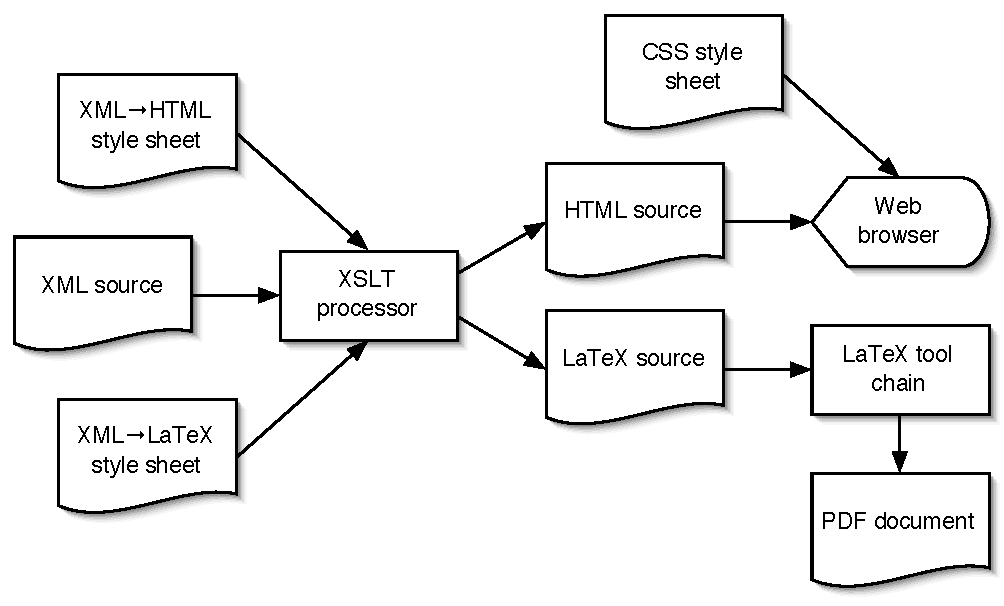
\includegraphics[height=6.5cm,keepaspectratio]{v1_workflow}
% 		
% 		\end{column}
% 		
% 	\end{columns}
% }
% 
% 
% \frame
% {
% 	\frametitle{But not all was well\ldots}
% 	
% 	\begin{itemize}
% 	
% 		\item Not designed for general documents (i.e., other than labs
% 		or tutorials).
% 	
% 		\item Two separate style sheets \(\Rightarrow\) harder to
% 		maintain consistency.
% 	
% 	\end{itemize}
% }
% 
% 
% \section[Version 2]{The second version of our authoring framework}
% 
% 
% \frame
% {
% 	\frametitle{\parbox[t]{\textwidth}{The second version of the framework \\
% 		\normalfont\tiny (2004)}}
% 	
% 	\begin{itemize}
% 	
% 		\item Single monolithic master format document combining both
% 		HTML and \LaTeX\ XSLT templates.
% 		
% 		\item Master format document processed through separate XSL
% 		master style sheets to produce XML \(\rightarrow\) HTML \&
% 		XML \(\rightarrow\) \LaTeX\ style sheets.
% 		
% 		\note{Nicely recursive---using a style sheet to generate style
% 		sheets!}
% 		
% 		\item Generalised to other types of documents.
% 	
% 	\end{itemize}
% }
% 
% 
% \frame
% {
% 	\frametitle{Workflow for version 2}
% 	
% 	\centering
% 	
% 	\begin{columns}
% 	
% 		\begin{column}{12cm}
% 	
% 			\centering
% 			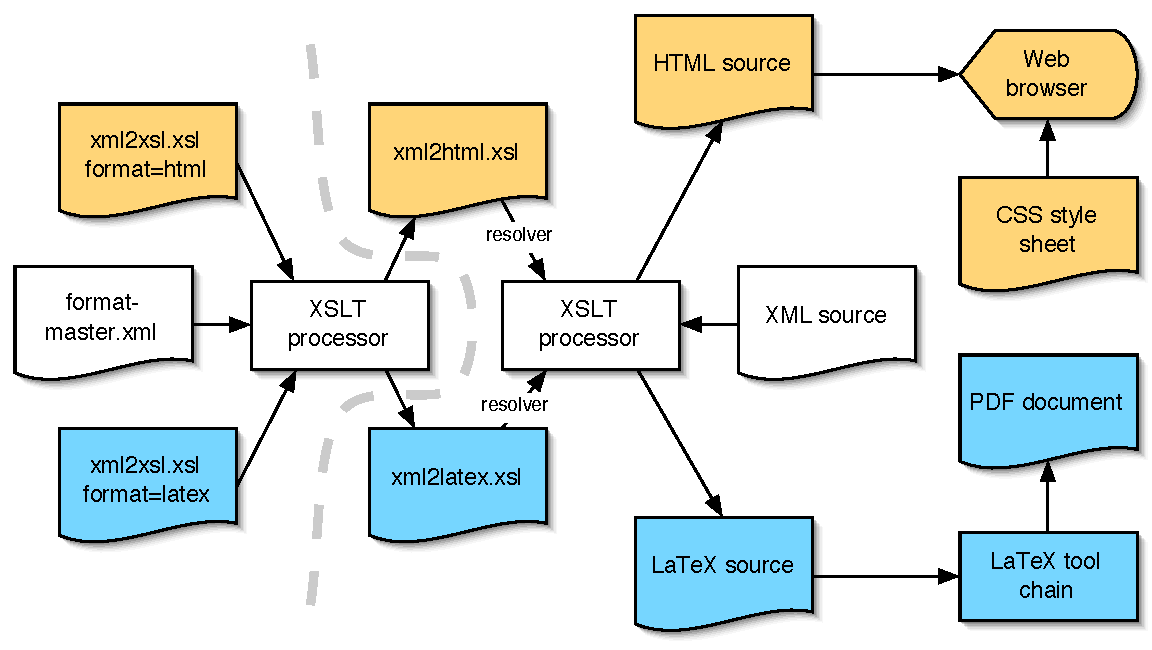
\includegraphics[height=6.5cm,keepaspectratio]{v2_workflow}
% 		
% 		\end{column}
% 		
% 	\end{columns}
% 	
% 	\note{Everything to the right of the thick dashed grey line is part
% 	of the day-to-day workflow. The stuff on the left on occurs when the
% 	master format is changed.}
% }
% 
% 
% \frame
% {
% 	\frametitle{Features}
% 	
% 	\begin{itemize}
% 	
% 		\item The usual paragraph formatting, etc.
% 		
% 		\item Moderately complex tabular structures (including
% 		multi-column \& multi-row cells).
% 		
% 		\item Hyperlinks \& cross-references.
% 		
% 		\item Floating matter (figures, tables).
% 		
% 		\note{Figures and tables don't float in HTML.}
% 		
% 		\item Images in various formats.
% 		
% 		\item \emph{Very} basic maths.
% 		
% 		\item Conditional processing based on format (\LaTeX/HTML).
% 	
% 		\item Raw code for that \emph{really} crufty stuff.
% 		
% 		\item etc\ldots
% 		
% 	\end{itemize}
% }
% 
% 
% \frame
% {
% 	\centering\Huge\alert{Examples}
% 	
% 	\note[item]{Show parts of format-master.xml and xml2xsl.xsl.}
% 	
% 	\note[item]{INFO 321 Analogy document (general document).}
% 	
% 	\note[item]{INFO 321 lab 3 is a good example of a lab document, with
% 	graphics, etc., plus it's embedded within the INFO 321 course
% 	handbook.}
% 	
% 	\note[item]{Do a clean build of the Analogy document and the
% 	handbook.}
% }
% 
% 
% \frame
% {
% 	\frametitle{BUT WHAT ABOUT DOCBOOK?}
% 	
% 	\begin{onlyenv}<2>
% 	
% 		\centering All right, all right!!
% 	
% 	\end{onlyenv}
% 	
% 	\begin{itemize}
% 	
% 		\item<3-> DocBook is a set of comprehensive SGML \& XSL style
% 		sheets for producing technical computing documents from XML
% 		source, managed by OASIS. {\scriptsize (see
% 		\texttt{http://www.docbook.org/})}
% 		
% 		\item<3-> Why didn't we use it? \uncover<4->{\alert<4>{We didn't know about
% 		it!}}
% 		
% 		\note<4>[item]{Also, it was a useful learning exercise to find
% 		out how XML + XSLT worked.}
% 		
% 		\item<5-> Our framework is remarkably similar but not quite as
% 		powerful.
% 		
% 		\note<5->[item]{For example, their tabulars are much more powerful!}
% 		
% 		\item<5-> But we seem to do some things a little better :)
% 		
% 		\note<5->[item]{For example, handling of special characters. Our handling
% 		of hyperlinks also seems a bit more flexible and intuitive.}
% 		
% 		\item<5-> Use formatting objects to output direct to PDF.
% 		
% 	\end{itemize}
% }
% 
% 
% \section[Problems]{Problems encountered}
% 
% 
% \frame
% {
% 	\frametitle{Problems encountered with version 2}
% 	
% 	\begin{itemize}
% 	
% 		\item Sometimes need to be careful about white space.
% 		
% 		\note[item]{For example, tabulars that followed each other in
% 		the source and were intended to be separate paragraphs, ended up
% 		on the same line in the PDF because the white space between them
% 		got eaten by the transformation.}
% 		
% 		\item Sometimes things just don't work \(\Rightarrow\) embedded
% 		raw code.
% 		
% 		\item \LaTeX-only vs.\ HTML-only features can be a nuisance.
% 		
% 		\item Master format document needs to be modularised.
% 		
% 		\note[item]{Master format is currently about 2000 lines.}
% 		
% 	\end{itemize}
% }
% 
% 
% \frame
% {
% 	\frametitle{Platform issues}
% 	
% 	\begin{itemize}
% 	
% 		\item Different \TeX\ distributions (fp\TeX\ vs.\ te\TeX).
% 		
% 		\note[item]{We now both use te\TeX.}
% 		
% 		\item Different XSLT processors (SAXON vs.\ Xalan-C vs.\
% 		Xalan-Java) with different command-line conventions.
% 		
% 		\note[item]{Solved the XSLT processor problem by defining an
% 		XSLT environment variable as appropriate on each machine, then
% 		defining a set of functions in our Makefiles to call the
% 		appropriate processor with the correct command line.}
% 		
% 		\item Line breaks!
% 		
% 		\note[item]{Line breaks pretty much resolved by storing
% 		everything in CVS.}
% 		
% 		\item Compatible vector drawing tools.
% 		
% 		\item Differing directory path conventions.
% 		
% 		\note[item]{Solved the path problem by using Cygwin on the Win32
% 		side.}
% 		
% 		\item Where to find the style sheets?
% 		
% 		\note[item]{Can resolve the style sheet location issue using
% 		either environment variables, symlinks or just copying the files
% 		into the local directory, but none of these are ideal. A nicer
% 		solution is to use the Apache XML-Commons resolver.}
% 	
% 	\end{itemize}
% }
% 
% 
% \section[Software]{What you need to do this yourself}
% 
% 
% \frame
% {
% 	\frametitle{The essential software}
% 	
% 	\begin{itemize}
% 	
% 		\item The XSL style sheets!
% 	
% 		\item XSLT processor (we use Apache Xalan or SAXON).
% 		
% 		\item A \TeX\ distribution (te\TeX).
% 		
% 		\item Something to edit XML with (GVim, BBEdit).
% 		
% 	\end{itemize}
% }
% 
% 
% \frame
% {
% 	\frametitle{Nice to have}
% 	
% 	\begin{itemize}
% 	
% 		\item GhostScript.
% 		
% 		\item GNU make.
% 		
% 		\item Vector drawing tool (Visio, OmniGraffle).
% 		
% 		\item Graphics manipulation tools (epstool, ImageMagick, \ldots).
% 		
% 		\item \LaTeX\ spelling checker (aspell, Excalibur).
% 		
% 		\item Version control (CVS).
% 		
% 		\note[item]{One nice feature of using CVS is that you can embed
% 		the CVS ID tags in the document so that you know which version
% 		of a document a student has.}
% 		
% 		\item Apache XML-Commons resolver for locating style sheets on
% 		the fly. {\scriptsize (see \texttt{http://xml.apache.org/commons/})}
% 		
% 		\note[item]{The resolver enables you to locate style sheets and
% 		DTDs on the fly using catalog files.}
% 	
% 	\end{itemize}
% }
% 
% 
% \section[Future]{Where to next?}
% 
% 
% \frame
% {
% 	\frametitle{Did we achieve our goals?}
% 	
% 	\begin{itemize}
% 	
% 		\item Cross-platform (Win32/Cygwin, Mac OS X, should work fine
% 		on any Unix derivative).
% 		
% 		\item \LaTeX\ gives high-quality print output.
% 		
% 		\item Good (and improving) HTML output.
% 		
% 		\item Customisable \& extensible.
% 		
% 		\item Sufficient geek factor :)
% 		
% 	\end{itemize}
% 	
% 	\begin{center}
% 	
% 		\uncover<2>{\Huge\alert{YES}}
% 	
% 	\end{center}
% }
% 
% 
% \frame
% {
% 	\frametitle{Beyond the current version}
% 	
% 	\begin{itemize}
% 	
% 		\item Roll out for INFO 212 (S2 2004).
% 		
% 		\item Investigate moving to DocBook (investigations in
% 		progress):
% 		
% 		\begin{itemize}
% 		
% 			\item Should be relatively easy to write an XSL style sheet
% 			to convert our markup to DocBook
% 			
% 			\item Need a customisation layer for ``our'' stuff
% 			
% 			\item Default PDF output too Word-like; also needs
% 			customisation (Apache FOP vs.\ Passive\TeX\ vs.\ ??)
% 			
% 		\end{itemize}
% 		
% 		\item Find a good cross-platform vector drawing tool! PGF?
% 		Sodipodi? Skencil? Kivio? Others? (but \alert{not} XFig!!!)
% 		
% 		\item SVG for graphics?
% 		
% 		\item Lecture slides in XML?
% 		
% 		\note{I can see advantages to having the lecture slides in XML,
% 		as it's going to be a lot easier to produce an HTML version from
% 		an XML original than from the \LaTeX/Beamer files that I have
% 		now.}
% 	
% 	\end{itemize}
% }
% 
% 
% \frame
% {
% 	\centering\Huge{\alert{Questions?}}
% }


\end{document}

%%%%%%%%%%%%%%%%%%%%%%%%%%%%%%%%%%%%%%%%%%%%%%%%%%%%%%%%%%%%%%%%%%%%%%%%%%%%%%%%
%
% $Log$
% Revision 1.4  2004/08/24 04:44:51  nstanger
% - Added history slides.
%
% Revision 1.3  2004/08/23 10:45:19  nstanger
% - Added initial section headings.
% - Started adding content.
% - Added timeline drawing macro.
%
% Revision 1.2  2004/08/23 05:03:46  nstanger
% - Added makefile (still broken).
% - Tweaked source to use driver approach.
% - Added some images.
%
% Revision 1.1.1.1  2004/08/23 00:30:26  nstanger
% - Added XML presentation.
%
%%%%%%%%%%%%%%%%%%%%%%%%%%%%%%%%%%%%%%%%%%%%%%%%%%%%%%%%%%%%%%%%%%%%%%%%%%%%%%%%
